\documentclass[12pt,a4paper]{book}
\usepackage{fullpage}
\usepackage{amsmath, amsthm, amssymb}
\usepackage{xltxtra,xgreek}
\usepackage{fontenc}
%\usepackage{backnaur}
\usepackage{verbatim}
\setmainfont{GFS Artemisia}
\usepackage{color}
\usepackage{enumitem}
\usepackage[pdfborder={0 0 0}]{hyperref}

\usepackage{graphicx}
\graphicspath{ {images_folder/} }
\usepackage{caption}
\usepackage{subcaption}
\usepackage{xltxtra} 
\usepackage{tabularx}
	


\title{Ανάπτυξη πρωτοτύπου συστήματος συγχρονισμένης συστοιχίας αισθητήρων υπερήχων (Ultrasonic Phased Array) βασισμένου σε FPGA, για χρήση σε μη καταστροφικό έλεγχο (NDT) υλικών}
\author{Μαρίνος Νικόλαος ΑΜ:2011506}
\date{Σεπτέμβριος 2014}

\begin{document}
{\Huge \maketitle}
\pagenumbering{arabic}
\tableofcontents

%%%%%%%%%%%%%%%%%%%%%%%%%%%%%%%%%%%%%%%%%%%%%%%%%%%%%%%%%%%%%%%%%%%%%%%%%%%%%%%%%%%%%%
%%%%%%%%%%%%%%%%%%%%%%%%ΚΕΦ 1: ΕΙΣΑΓΩΓΗ%%%%%%%%%%%%%%%%%%%%%%%%%%%%%%%%%%%%%%%%%%%%%%%
%%%%%%%%%%%%%%%%%%%%%%%%%%%%%%%%%%%%%%%%%%%%%%%%%%%%%%%%%%%%%%%%%%%%%%%%%%%%%%%%%%%%%%
\chapter{Εισαγωγή}
\section{field-programmable gate array (FPGA)}
Ένα FPGA είναι ειδικού τύπου ολοκληρωμένα κύκλωμα, των οποίων η εσωτερική δομή και κατ'επεκταση, η λειτουργία τους, μπορεί να ρυθμιστεί μετά την παραγωγή τους σε αντίθεση με τα ASIC. Αποτελούνται από ένα μεγάλο αριθμό στοιχείων προγραμματιζόμενης λογικής και από ένα επαναρυθμιζόμενο δίκτυο διασυνδέσεων μεταξύ τους. Τα στοιχεία αυτά μπορούν να ρυθμιστούν ώστε να εκτελούν απλές λειτουργίες, όπως μία πύλη AND ή πιο σύνθετες συνδυαστικές λογικές. Επίσης στα FPGA υπάρχουν και στοιχεία μνήμης καθώς και άλλα κυκλώματα σχεδιασμένα να εκτελούν συγκεκριμένες λειτουργίες. Συνδυάζοντας όλα τα παραπάνω μπορούν να αναπτυχθούν πολύπλοκα συστήματα τα οποία να εκτελούν κάποια εξειδικευμένη λειτουργία.

Η χρήση των FPGA για την ανάπτυξη ενός συστήματος έχει μεγάλα πλεονεκτήματα συγκριτικά με τη χρήση εξειδικευμένων ολοκληρωμένων κυκλωμάτων (ASIC). Τα σημαντικότερα πλεονεκτήματα είναι η ταχύτητα ανάπτυξης του συστήματος και το πολύ χαμηλότερο κόστος. Η κατασκευή ενός καινούριου ASIC έχει τεράστιο κόστος, κάνοντας τη χρήση του σχεδόν απαγορευτική κατά τη διάρκεια της ανάπτυξης ενός συστήματος. Αντίθετα τα FPGA είναι πολύ πιο φτηνά και μπορούν να ξαναχρησιμοποιηθούν σε περίπτωση που αναπτυχθεί νέα έκδοση του συστήματος.

Υπάρχουν δύο τρόποι ανάπτυξης τέτοιων συστημάτων. Ο πρώτος (χρονικά) που χρησιμοποιήθηκε ήταν ο γραφικός (σχηματικός). Το σύστημα σχεδιαζόταν ως κύκλωμα πυλών και άλλων στοιχείων. Σύντομα όμως η πολυπλοκότητα των συστημάτων μεγάλωσε τόσο, που δεν ήταν δυνατός ο σχεδιασμός τους με αυτόν τον τρόπο. Τότε άρχισαν να χρησιμοποιούνται οι γλώσσες περιγραφής υλικού (Hardware Description Languages - HDL). Οι πιο διαδεδομένες είναι η VHDL και η Verilog. Με τη βοήθεια αυτών των γλωσσών μπορεί να επιτευχθεί η ανάπτυξη περίπλοκων και μεγάλων συστημάτων σε πολύ μικρότερο χρόνο.

Οι γλώσσες αυτές επιτρέπουν την περιγραφή της δομής ενός συστήματος ή της επιθυμητής συμπεριφοράς του. Στη συνέχεια τα εργαλεία (synthesizers) φροντίζουν για την μετάφραση αυτής της περιγραφής σε μία διάταξη υλικού η οποία να έχει τη συμπεριφορά που καθορίσαμε και να μπορεί να υλοποιηθεί στο FPGA που θα χρησιμοποιηθεί. Τα εργαλεία αυτά παρέχονται από τις εταιρίες που κατασκευάζουν FPGA.

Μερικές εταιρίες κατασκευής FPGA είναι η Xilinx, η Altera, η Microsemi, η Tabula, η Lattice Semiconductor κ.α. με τις δύο πρώτες να έχουν το μεγαλύτερο μερίδιο της αγοράς.

Τα τελευταία χρόνια οι κατασκευαστές αυτοί έχουν στραφεί και στη δημιουργία ολόκληρων συστημάτων πάνω σε ένα ολοκληρωμένο κύκλωμα (System on Chip - SoC). Τα συστήματα αυτά συνδυάζουν προγραμματιζόμενη λογική, επεξεργαστές και άλλα στοιχεία πάνω στο ίδιο ολοκληρωμένο. Η συνύπαρξή τους στο ίδιο ολοκληρωμένο κάνει την αλληλεπίδραση μεταξύ των στοιχείων αυτών πολύ εύκολη.

%Ένα τέτοιο SoC είναι το Xilinx Zynq-7000, το οποίο συνδυάζει ένα Artix-7 FPGA με έναν διπύρηνο ARM Cortex A9. Η επικοινωνία μεταξύ της προγραμματιζόμενης λογικής και του επεξεργαστή και της μνήμης γίνεται μέσω έτοιμων θυρών, οι οποίες χρησιμοποιούν το Advanced eXtensible Interface 4 (AXI4) πρωτόκολλο το οποίο είναι μέρος του Advanced Microcontroller Bus Architecture (AMBA). Το πρωτόκολλο αυτό είναι ανοιχτού κώδικα και υποστηρίζεται από την ARM.  


\section{Μη καταστροφικός έλεγχος (NDT)}
Μη καταστροφικός έλεγχος είναι ένα ευρύ σύνολο τεχνικών και τεχνολογιών που χρησιμοποιούνται στην επιστήμη και τη βιομηχανία για την αξιολόγηση ιδιοτήτων υλικών και συστημάτων χωρίς την καταστροφή τους. Οι τεχνικές αυτές βασίζονται στη χρήση ηλεκτρομαγνητικής ακτινοβολίας, ήχου και άλλων φυσικών φαινομένων για τον εντοπισμό ατελειών ή βλαβών στα υλικά. Μερικές από αυτές τις τεχνικές είναι οι ακόλουθες:
\begin{itemize}
\item Έλεγχος ακουστικής εκπομπής (acoustic emmition)
\item Ηλεκτρομαγνητικός έλεγχος
\item Eddy-current testing
\item Δοκιμές καθοδηγούμενων κυμάτων (guided waves)
\item Υπέρυθρος και θερμικός έλεγχος
\item Ραδιογραφία
\item Έλεγχος με υπερήχους
\item Ανάλυση κραδασμών
\end{itemize}

Όλες οι μεγάλες βιομηχανίες χρησιμοποιούν τέτοιες τεχνικές για την πρόληψη εμφάνισης βλαβών στα συστήματά τους και τον ποιοτικό έλεγχο των προϊόντων τους. Ενδεικτικά μερικές εφαρμογές:
\begin{itemize}
\item επαλήθευση συγκολλήσεων 
\item εντοπισμός ρωγμών σε σωλήνες μεταφοράς πετρελαίου
\item έλεγχος εσωτερικής διάβρωσης σωλήνων νερού
\item παρακολούθηση ανεμογεννήτριας για εμφάνιση ρωγμών καταπόνησης
\item παρακολούθηση φθορών σε ράγες σιδηροδρόμων
\end{itemize}
Με τη βοήθεια αυτών των τεχνικών μπορεί να υπολογιστεί ο χρόνος ζωής ενός αντικειμένου ή να προβλεφθεί κάποια αστοχία του. Με αυτό τον τρόπο μπορεί να προληφθεί η όποια καταστροφή, επισκευάζοντας ή αντικαθιστώντας το κρίσιμο αντικείμενο. Αυτό μειώνει κατά πολύ το κόστος, μιας και μία αστοχία μπορεί να προκαλέσει το κλείσιμο μιας ολόκληρης μονάδας παραγωγής, και φυσικά εξαλείφει τον κίνδυνο ατυχήματος.

Στα πλαίσια της εργασίας αυτής ασχοληθήκαμε με τον μη καταστροφικό έλεγχο με τη βοήθεια των υπερήχων για χρήση κυρίως σε μέταλλα.



\section{Συγχρονισμένη συστοιχία υπερήχων (Ultrasonic Phased array)}
Τα συμβατικά συστήματα υπερήχων συνήθως αποτελούνται από έναν μετατροπέα (transducer) υπερήχων που δουλεύει ως πομπός και από έναν δεύτερο που δουλεύει ως δέκτης. Ο πομπός παράγει παλμούς υπερήχων οι οποίοι διαδίδονται μέσα στο υλικό που θέλουμε να ελέγξουμε. Ως πομποί χρησιμοποιούνται ειδικοί transducers οι οποίοι έχουν αρκετά καλή κατευθυντικότητα. Παράγουν δηλαδή δέσμες υπερήχων που διαδίδονται σε μία συγκεκριμένη κατεύθυνση. Ο δέκτης τοποθετείται σε κατάλληλο σημείο ώστε να λαμβάνει τους υπερήχους αφού περάσουν μέσα από το υλικό, καθώς και τις όποιες ανακλάσεις τους. Οι ανακλάσεις αυτές μπορεί να προέρχονται από τις επιφάνειες του υλικού ή από εσωτερικές ατέλειες όπως ρωγμές και τρύπες. Ξέροντας τη γεωμετρία του υλικού και τα σημεία που έχουν τοποθετηθεί οι transducers, μπορούμε να υπολογίσουμε την αναμενόμενη πορεία των παλμών και το τι θα πρέπει να λαμβάνει ο δέκτης. Αν τα αποτελέσματά μας διαφέρουν από τα αναμενόμενα σημαίνει πως κάποια ατέλεια υπάρχει στο εσωτερικό του υλικού. 

Ένα τέτοιο παράδειγμα φαίνεται στην εικόνα \ref{single_elem_transd}. Ο υπέρηχος διαδίδεται ως δέσμη στο υλικό και ανακλάται από την διεπαφή του transducer με το υλικό, τις τρύπες και από την επιφάνειά του στο κάτω μέρος (backwall). Στην εικόνα \ref{a_scan} βλέπουμε μία απεικόνιση των ανακλάσεων. Αυτού του είδους η απεικόνιση ονομάζεται A scan.

\begin{figure}
	\centering
	\begin{subfigure}[b]{0.4\textwidth}
		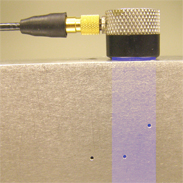
\includegraphics[width=\textwidth]{single_elem_transd}
		\caption{transducer ενός στοιχείου}
		\label{single_elem_transd}
	\end{subfigure}	
	\begin{subfigure}[b]{0.4\textwidth}
		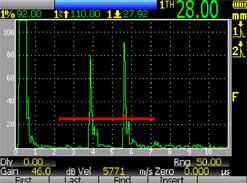
\includegraphics[width=\textwidth]{a_scan}
		\caption{A scan}
		\label{a_scan}
	\end{subfigure}
	\caption{Συμβατικό σύστημα υπερήχων}
\end{figure}

Όπως μπορούμε να παρατηρήσουμε στο παραπάνω A scan, η χρήση ενός μόνο transducer μπορεί να μας δώσει πληροφορία για την ύπαρξη μίας ατέλειας στο υλικό και για την απόστασή της από αυτόν. Δεν μπορούμε όμως να καταλάβουμε την ακριβή θέση και το σχήμα της. Για αυτό το λόγο κατασκευάστηκαν συστοιχίες από transducers. Οι συστοιχίες αυτές αποτελούνται από 8 ή μέχρι και 256 μετατροπείς υπερήχων \ref{32el_PA}. Ο κάθε ένας από αυτούς είναι μικρός σε μέγεθος και μπορεί να παράγει παλμούς υπερήχων. Λόγω όμως του μικρού τους μεγέθους, οι transducers αυτοί έχουν πολύ μικρότερη κατευθυντικότητα σε σχέση με αυτούς μεγαλήτερου μεγέθους. Ως αποτέλεσμα, οι υπέρηχοι δεν διαδίδονται ως δέσμες, αλλά ως σφαιρικά κύματα. Το πλήθος όμως των στοιχείων μας επιτρέπει να χρησιμοποιήσουμε τεχνικές που αξιοποιούν ιδιότητες των ηχητικών κυμάτων, με κυριότερη τη συμβολή κυμάτων, για να δημιουργήσουμε μία πολύ καλή απεικόνιση των εσωτερικών ατελειών.

\begin{figure}
	\centering
	
\includegraphics[width=0.4\textwidth]{myimage}
	\caption{32 elements phased array probe}
	\label{32el_PA}
\end{figure}

Στην εργασία αυτή θα χρησιμοποιήσουμε δύο τέτοιες τεχνικές. Η πρώτη ονομάζεται full matrix capture (FMC). Στην τεχνική αυτή ένα από τα στοιχεία στέλνει έναν παλμό υπερήχων και όλα τα στοιχεία λαμβάνουν τις ανακλάσεις. Η διαδικασία επαναλαμβάνεται για όλα τα στοιχεία της συστοιχίας. Όταν τελειώσει η ακολουθία μεταδόσεων - λήψεων, έχοντας όλα τα δεδομένα στη διάθεσή μας, μπορούμε να χρησιμοποιήσουμε έναν κατάλληλο αλγόριθμο (total focusing method - TFM) για τον συνδυασμό των δεδομένων και την δημιουργία μιας λεπτομερής απεικόνισης της περιοχή ελέγχου.

Η δεύτερη τεχνική λέγεται διαμόρφωση δέσμης (beamforming) και έχει δύο στάδια. Το πρώτο είναι η διαμόρφωση κατά την εκπομπή των παλμών υπερήχων και το δεύτερο η διαμόρφωση κατά τη λήψη. Η διαμόρφωση αυτή, εκμεταλλεύεται τη συμβολή των κυμάτων για τη δημιουργία μίας δέσμης υπερήχων η οποία εστιάζει σε ένα συγκεκριμένο σημείο του υλικού που θέλουμε να ελέγξουμε και επιτυγχάνεται εκπέμποντας παλμούς από πολλούς transducers ταυτόχρονα, αλλά με μικρές διαφορές φάσης μεταξύ τους. Με κατάλληλα υπολογισμένες διαφορές, μπορούμε να προκαλέσουμε δημιουργική συμβολή στο σημείο που θέλουμε και καταστροφική στη γύρω περιοχή. Με αυτόν τον τρόπο δημιουργούμε μία κατευθυνόμενη δέσμη υπερήχων όπως φαίνεται στο σχέδιο \ref{tx_bfm}. . Αλλάζοντας τη διαμόρφωση, μπορούμε να αλλάξουμε και κατεύθυνση της δέσμης και το βάθος εστίασης. 



\begin{figure}
	\centering
	
\includegraphics[width=0.4\textwidth]{myimage}
	\caption{transmit beamforning}
	\label{tx_bfm}
\end{figure}

Στη συνέχεια, όλα τα στοιχεία λαμβάνουν τους ανακλώμενους υπερήχους. Τα σήματα αυτά, μετά τη λήψη τους, μετατοπίζονται χρονικά σύμφωνα με τις αντίστοιχες καθυστερήσεις μεταξύ των εκπεμπόμενων παλμών και αθροίζονται. Αυτή η διαδικασία ονομάζεται receive beamforming ή διαμόρφωση δέσμης κατά τη λήψη και ουσιαστικά είναι η αντίστροφη διαδικασία από το transmit beamforming.  Το τελικό σήμα χρησιμοποιείται για τη δημιουργία της απεικόνισης της εσωτερικής δομής του υλικού στην κατεύθυνση της δέσμης. Επαναλαμβάνοντας τη διαδικασία με διαφορετικούς χρονισμούς μπορούμε να δημιουργήσουμε νέα δέσμη με διαφορετική κατεύθυνση. Με αυτόν τον τρόπο μπορούμε να πραγματοποιήσουμε γραμμική σάρωση (linear scan - B-scan)(εικόνες \ref{linear_scan} και \ref{b_scan}) ή σάρωση τομέα (sectorial scan - S-scan) (εικόνες \ref{sectorial_scan} και \ref{s_scan}) του δείγματος που ελέγχουμε, χωρίς να χρειαστεί να μετακινήσουμε καθόλου τον αισθητήρα.

\begin{figure}
	\centering
	\begin{subfigure}[b]{0.4\textwidth}
		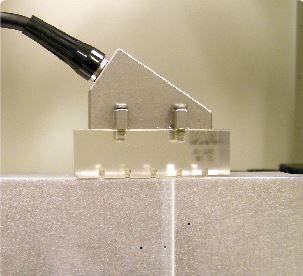
\includegraphics[width=\textwidth]{linear_scan}
		\caption{γραμμική σάρωση}
		\label{linear_scan}
	\end{subfigure}	
	\begin{subfigure}[b]{0.4\textwidth}
		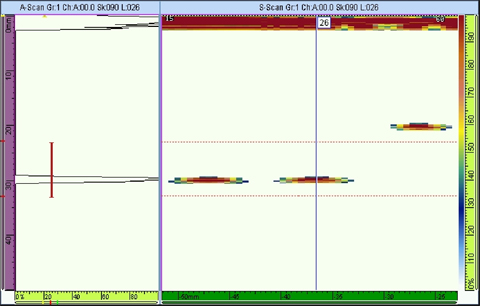
\includegraphics[width=\textwidth]{b_scan}
		\caption{B scan}
		\label{b_scan}
	\end{subfigure}
	\begin{subfigure}[b]{0.4\textwidth}
		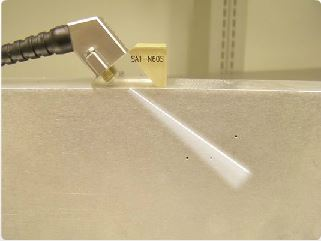
\includegraphics[width=\textwidth]{sectorial_scan}
		\caption{γωνιακή σάρωση}
		\label{sectorial_scan}
	\end{subfigure}	
	\begin{subfigure}[b]{0.4\textwidth}
		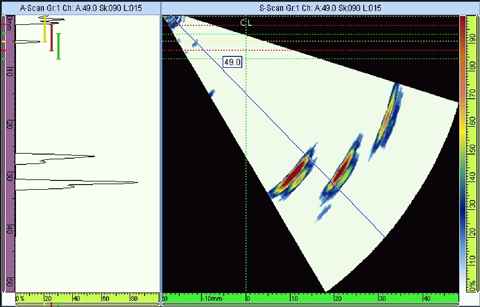
\includegraphics[width=\textwidth]{s_scan}
		\caption{S scan}
		\label{s_scan}
	\end{subfigure}
	\caption{μέθοδοι phased array scanning}
\end{figure}

\chapter{Γενική περιγραφή και απαιτήσεις συστήματος}
Το σύστημα υπερήχων που αναπτύξαμε αποτελείται από δύο μέρη. Το ψηφιακό και το αναλογικό. Το πρώτο έχει σχεδιαστεί πάνω στο SoC και είναι υπεύθυνο για τον έλεγχο του αναλογικού κομματιού του συστήματος, για τη λήψη των δεδομένων και για την επεξεργασία τους. Αποτελεί το κυρίως μέρος της διπλωματικής αυτής. Το αναλογικό κομμάτι έχει να κάνει με την παραγωγή των υπερήχων, τη λήψη τους και τη μετατροπή τους τελικά σε ψηφιακό σήμα. Στο σχήμα \ref{syst_schem} μπορούμε να δούμε το σχεδιάγραμμα του συστήματος και την ροή της λειτουργίας του.

\begin{figure}
	\centering
	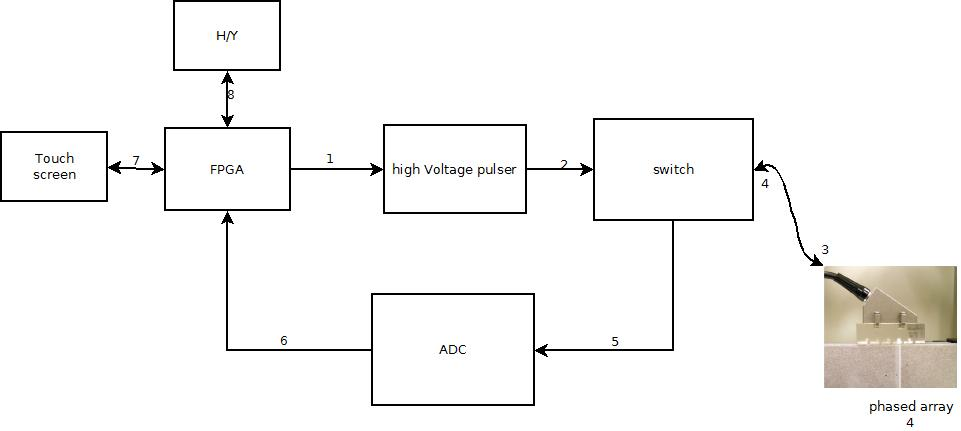
\includegraphics[width=\textwidth]{system_schem}
	\caption{Σχεδιάγραμμα συστήματος}
	\label{syst_schem}
\end{figure}

Αρχικά το FPGA παράγει κατάλληλα σήματα για την οδήγηση όλων των pulsers. Οι pulsers παράγουν τους παλμούς υψηλής τάσης, ανάλογα με τα σήματα που δέχονται. Στη συνέχεια οι παλμοί κατευθύνονται στους transducers του phased array, αφού περάσουν από ένα switch. Το switch προστατεύει το κύκλωμα κατευθύνοντας την υψηλή τάση προς τους trasnducers και όχι προς τον ADC. Οι παλμοί διεγείρουν τους transducers και οι παλμοί υπερήχων παράγονται. Οι υπέρηχοι διαδίδονται μέσα στο υλικό και αφού ανακλαστούν επιστρέφουν στους transducers. Εκεί μετατρέπονται σε ηλεκτρικό σήμα το οποίο κατευθύνεται στον ADC για ψηφιοποίηση. Ο switch φροντίζει για τη δρομολόγηση του προς τον ADC. Τέλος το ψηφιοποιημένο σήμα στέλνεται στο FPGA για επεξεργασία και αποθήκευση. 

Στο FPGA υπάρχει συνδεδεμένη μία οθόνη αφής. Με αυτή μπορεί να πραγματοποιηθεί ένας βασικός έλεγχος του συστήματος και επίσης γίνεται και η απεικόνιση των δεδομένων. Επίσης το σύστημα είναι συνδεδεμένο με έναν υπολογιστή μέσω ethernet για την αποστολή των δεδομένων σε αυτόν και για τον πιο λεπτομερή έλεγχο των λειτουργιών του.

Πιο συγκεκριμένα, για την ανάπτυξη του συστήματος χρησιμοποιήσαμε τα ακόλουθα:
\begin{itemize}
	\item Zedboard (Zynq Evaluation and Development Board)
	\item MAX4940 quad bipolar high voltage digital pulser (x2)
	\item ultrasonic phased array: IMASONIC 5Mhz - 32elts
	\item ανακατευθυντής ηλεκτρικών σημάτων (switch): MAX4936A
	\item μετατροπέας αναλογικού σήματος σε ψηφιακό 8 καναλιών (analog to digital converter - ADC): AD9279
	\item οθόνη αφής: 7-inch Zed Touch Display Kit
	\item υπολογιστής
	\item τροφοδοτικό υψηλών και χαμηλών τάσεων
\end{itemize}

Αρχικά η ανάπτυξη του συστήματος πραγματοποιήθηκε με τη χρήση έτοιμων δοκιμαστικών πλακετών (development/evaluation boards) που παρέχουν οι εταιρίες που κατασκευάζουν τα ολοκληρωμένα κυκλώματα. Το σύστημα που αναπτύχθηκε τελικά βασίζεται σε πλακέτα που σχεδιάστηκε ειδικά για το σύστημα. Στην πλακέτα αυτή ενσωματώθηκαν όλα τα ολοκληρωμένα κυκλώματα εκτός από το SoC. 

Μέρος της εργασίας αυτής, εκτός από τον σχεδιασμό του ψηφιακού μέρους του συστήματος, ήταν και ο έλεγχος της ορθής λειτουργίας της πλακέτας αυτής.

Στα επόμενα υποκεφάλαια ακολουθεί παρουσίαση των υποσυστημάτων που χρησιμοποιήθηκαν.
\section{Περιγραφή υποσυστημάτων}

\subsection{Zedboard}
Το Zedboard (Zynq Evaluation and Development Board) είναι ένα σύστημα βασισμένο στο Xilinx Zynq$ ^{TM} $ -7000 All Programmable SoC και πιο συγκεκριμένα στο Xilinx$ ^{®} $ XC7Z020 System on Chip. Το chip αυτό συνδυάζει έναν διπύρηνο Corex-A9 επεξεργαστή της ARM (Processing System - PS) με ένα Artix-7 FPGA της Xilinx (αναφερόμενο και ως Programmable Logic - PL) μέσα σε ένα ολοκληρωμένο κύκλωμα. 

Η συνύπαρξή αυτών των δύο επιτρέπει την πολύ εύκολη αλληλεπίδρασή τους μέσω των ήδη έτοιμων interfaces. Τα interfaces αυτά ακολουθούν το πρότυπο AXI. Το πρότυπο αυτό έχει καθιερωθεί στη βιομηχανία διότι δίνει πολύ μεγάλη ευελιξία στη σύνδεση περιφεριακών με τον επεξεργαστή και μεταξύ τους. Στην εικόνα \ref{zynq7020} μπορούνε να δούμε την αρχιτεκτονική του Zynq 7020. Παρατηρούμε ότι ο επεξεργαστής είναι απευθείας συνδεδεμένος με ένα μεγάλο πλήθος έτοιμων περιφεριακών, καθιστώντας πολύ εύκολη και γρήγορη την ανάπτυξη συστημάτων. Για παράδειγμα υπάρχουν έτοιμοι controllers για Ethernet (με DMA) και UART, κάτι που θα αξιοποιήσουμε στο σύστημά μας.
\begin{figure}
	\centering
	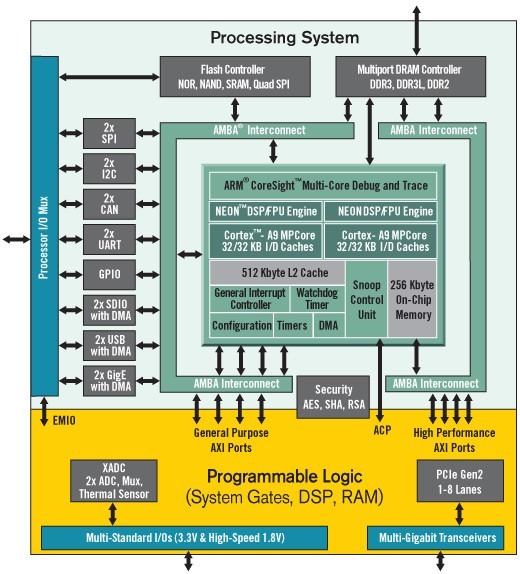
\includegraphics[width=\textwidth]{zynq7020}
	\caption{Σχεδιάγραμμα Zynq 7020}
	\label{zynq7020}
\end{figure}
Ταυτόχρονα, όπως προαναφέρθηκε, έχουμε μεγάλο αριθμό interfaces που ενώνουν το PS με την PL. Συγκεκριμένα, έχουμε δύο είδη. Το πρώτο είναι οι General purpose (γενικής χρήσης) AXI ports που είναι κατάλληλες για τη σύνδεση του επεξεργαστή με περιφερειακά που έχουμε σχεδιάσει στην programmable logic. Μέσω αυτών ο επεξεργαστής βλέπει τους εσωτερικούς registers των περιφερειακών μας ως επέκταση της μνήμης του. Το κάθε περιφερειακό καταλαμβάνει συγκεκριμένες διευθύνσεις. Με αυτόν τον τρόπο μπορούμε να έχουμε πολύ εύκολο έλεγχο των συστημάτων που σχεδιάζουμε. 
Το δεύτερο είναι οι High Performance AXI ports, οι οποίες έχουν απευθείας σύνδεση με τις μνήμες (DDR και on-chip) χωρίς την παρέμβαση του επεξεργαστή. Με αυτόν τον τρόπο τα διάφορα συστήματα που έχουμε σχεδιάσει στην PL έχουν άμεση πρόσβαση (DMA) σε αυτές και μάλιστα με πολύ μεγάλο bandwidth (πάνω από 4GBps).  

Το Zynq 7020 βρίσκεται πάνω σε μία πλακέτα (εικόνα \ref{zedboard}) μαζί με αρκετά έτοιμα περιφερειακά και interfaces όπως led, κουμπιά, διακόπτες, υποδοχή για sd card, 2 x ddr3 512 MB, PMOD, FMC κ.α. Αυτά είναι συνδεδεμένα ή με τον επεξεργαστή ή με την προγραμματιζόμενη λογική όπως φαίνεται και στην εικόνα \ref{zed_periph}.
\begin{figure}
	\centering
	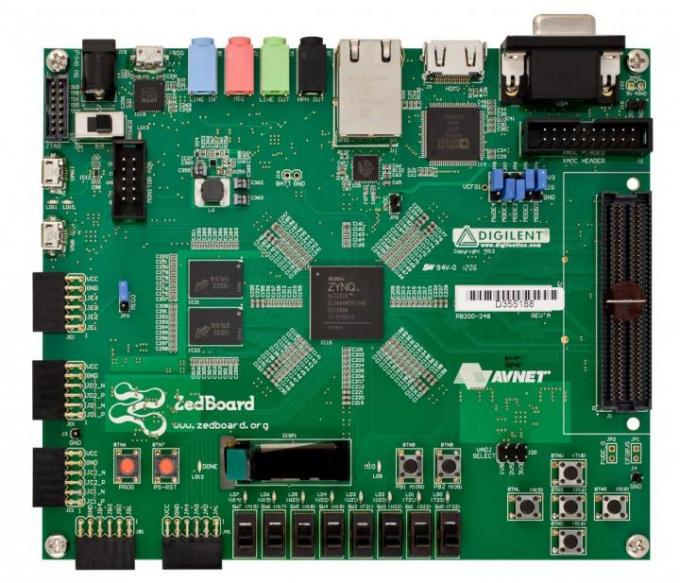
\includegraphics[width=\textwidth]{zedboard}
	\caption{Zedboard}
	\label{zedboard}
\end{figure}

\begin{figure}
	\centering
	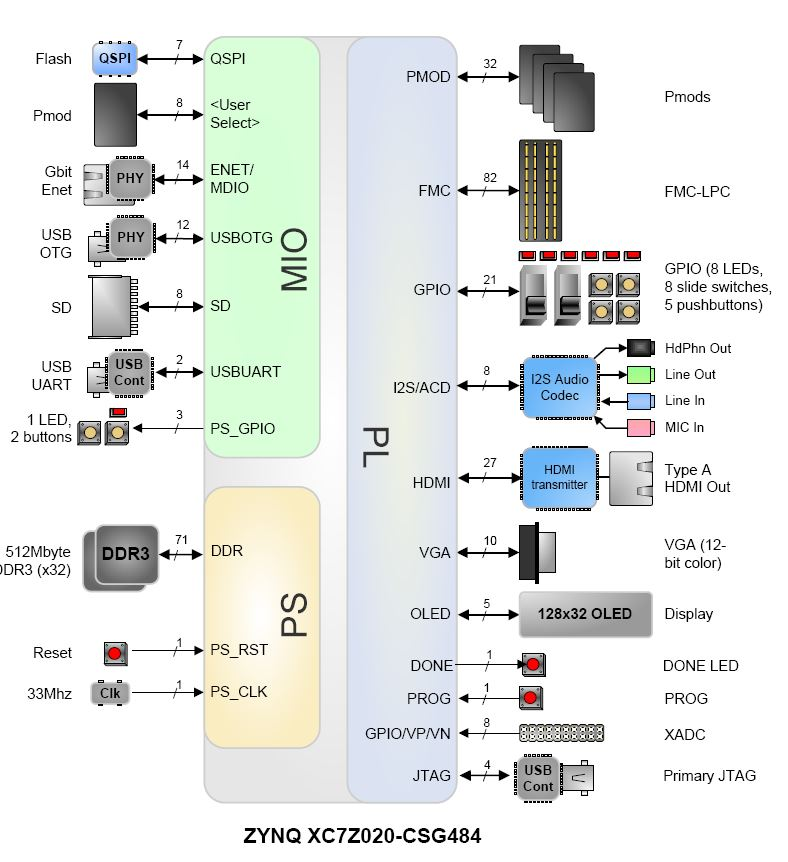
\includegraphics[width=\textwidth]{zed_periph}
	\caption{Zedboard block diagram}
	\label{zed_periph}
\end{figure}


\subsection{7-inch Zed Touch Display kit}
Η χρήση του συστήματος απαιτεί την άμεση απεικόνιση των δεδομένων. Ταυτόχρονα απαιτείται και η δυνατότητα απλού ελέγχου. Μια οθόνη αφής είναι ιδανική για τέτοια χρήση. Για αυτό θα χρησιμοποιηθεί το 7-inch Zed Touch Display kit της AVNET (εικ \ref{zed_touch}), το οποίο είναι συμβατό με το Zedboard. Η σύνδεση με το Zedboard γίνεται μέσω των PMOD και υπάρχουν έτοιμοι controllers για χρήση στο FPGA σύστημά μας.
\begin{figure}
	\centering
	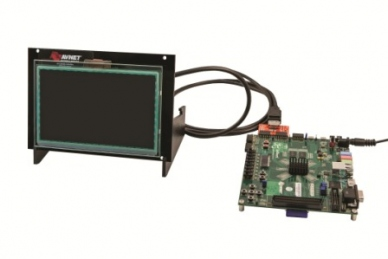
\includegraphics[width=\textwidth]{zed_touch}
	\caption{7-inch Zed Touch Display kit}
	\label{zed_touch}
\end{figure}

\subsection{MAX4940 evaluation board}
To MAX4940 της MAXIM είναι μία τετρακάναλη, ψηφιακή παλμογεννήτρια (pulser) η οποία μπορεί να παράξει διπολικούς παλμούς υψηλής τάσης και υψηλής συχνότητας, από χαμηλής τάσης σήματα. Οι παλμοί εξόδου μπορούν να είναι μέχρι και $ \pm $110V, ανάλογα φυσικά με την τάση τροφοδοσίας. Στο δικό μας σύστημα θα χρησιμοποιήσουμε τάση $ \pm $70V. Για την δημιουργία των διπολικών παλμών απαιτούνται 3 σήματα ανά κανάλι, ένα για τον θετικό παλμό, ένα για τον αρνητικό και ένα για το clamp, την επιστροφή δηλαδή στο μηδέν. Χρησιμοποιώντας αυτά τα σήματα μπορούμε να δημιουργήσουμε οποιαδήποτε ακολουθία παλμών θέλουμε.

Η πλακέτα με το MAX4940 φαίνεται στην εικόνα \ref{max4940}. Το πρωτότυπό που αναπτύσσουμε είναι οχτακάναλο, άρα θα χρησιμοποιήσουμε δύο τέτοιες πλακέτες, οι οποίες θα συνδέονται με τα PMOD ports του Zedboard. 
\begin{figure}
	\centering
	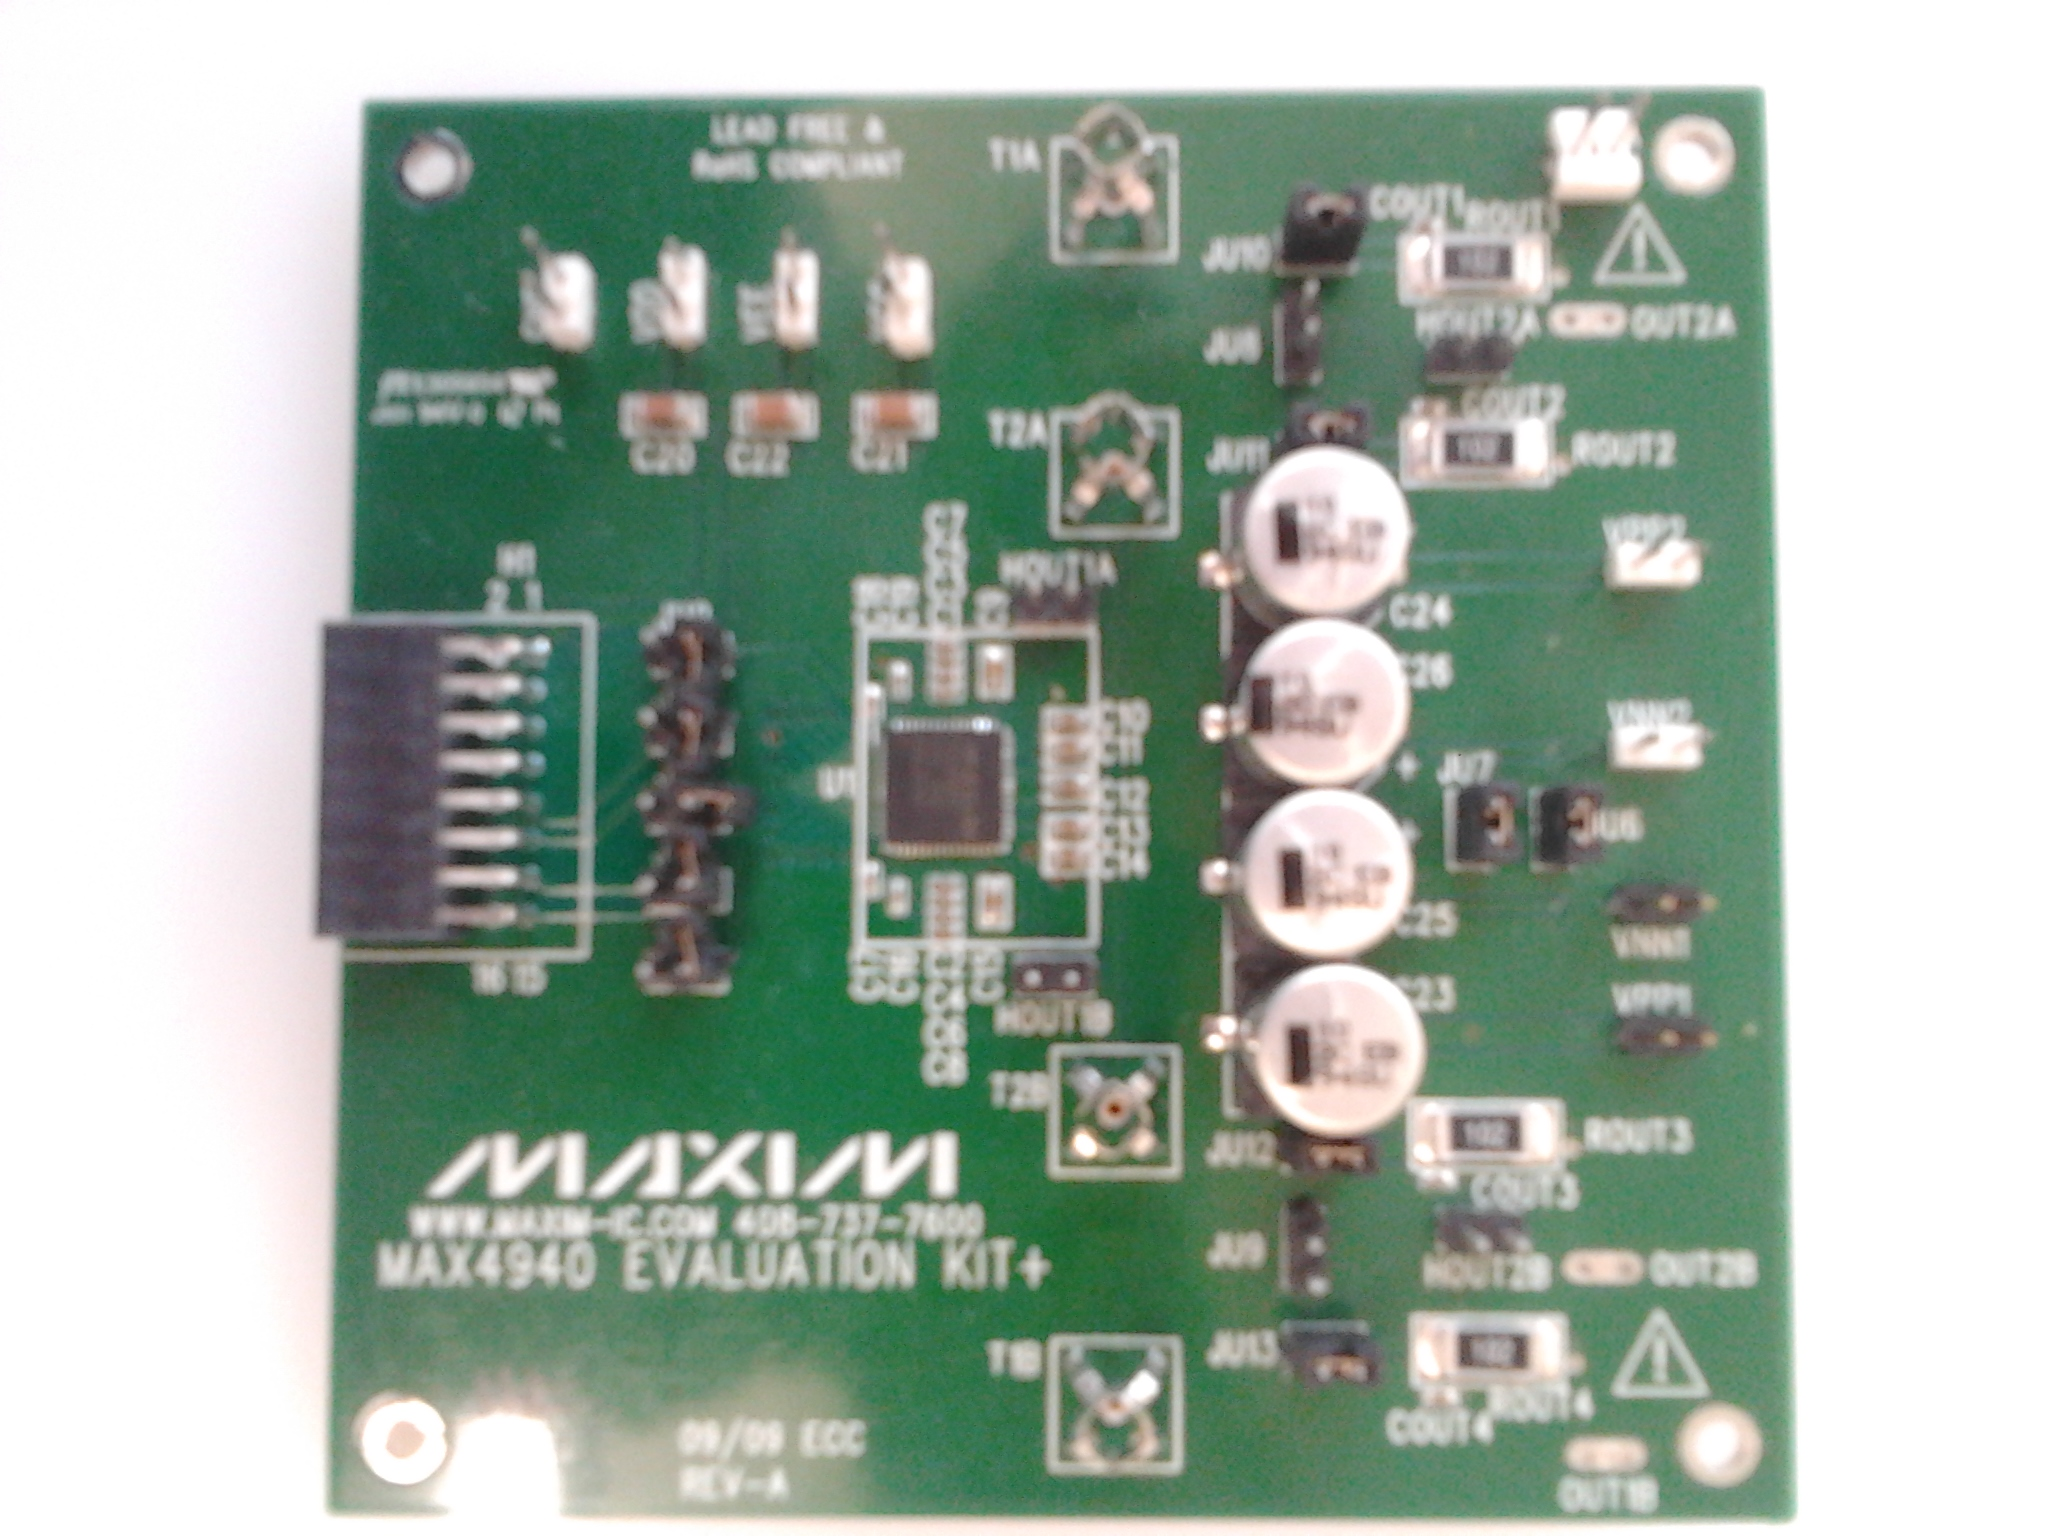
\includegraphics[width=\textwidth]{max4940}
	\caption{MAX4940 evaluation board}
	\label{max4940}
\end{figure}

\subsection{AD9279 evaluation board}
Ο AD9279 (εικ. \ref{ad9279}) είναι ένας οχτακάναλος μετατροπέας αναλογικού σήματος σε ψηφιακό (ADC). Συμπεριλαμβάνει επίσης ρυθμιζόμενα φίλτρα και ενισχυτές σήματος. Η δειγματοληψία μπορεί να γίνει με ρυθμό μέχρι 80 Msps. Στο σύστημα που αναπτύξαμε στο FPGA φροντίσαμε ώστε να μπορούμε να πετύχουμε αυτή την ταχύτητα. Αλλά στο αρχικό πρωτότυπο η συχνότητα δειγματοληψίας 65 Msps διότι ο AD9729 πάνω στο evaluation board είναι συνδεδεμένος με κρύσταλλο που παράγει ρολόι 65 Mhz.Η ψηφιοποίηση κάθε καναλιού γίνεται με ακρίβεια 12 bits τα οποία μεταδίδονται σειριακά στο FPGA. Η πλακέτα αυτή συνδέεται με το FMC (Low Pin Count - LPC) του Zedboard, με τη βοήθεια ενός interposer.

\begin{figure}
	\centering
	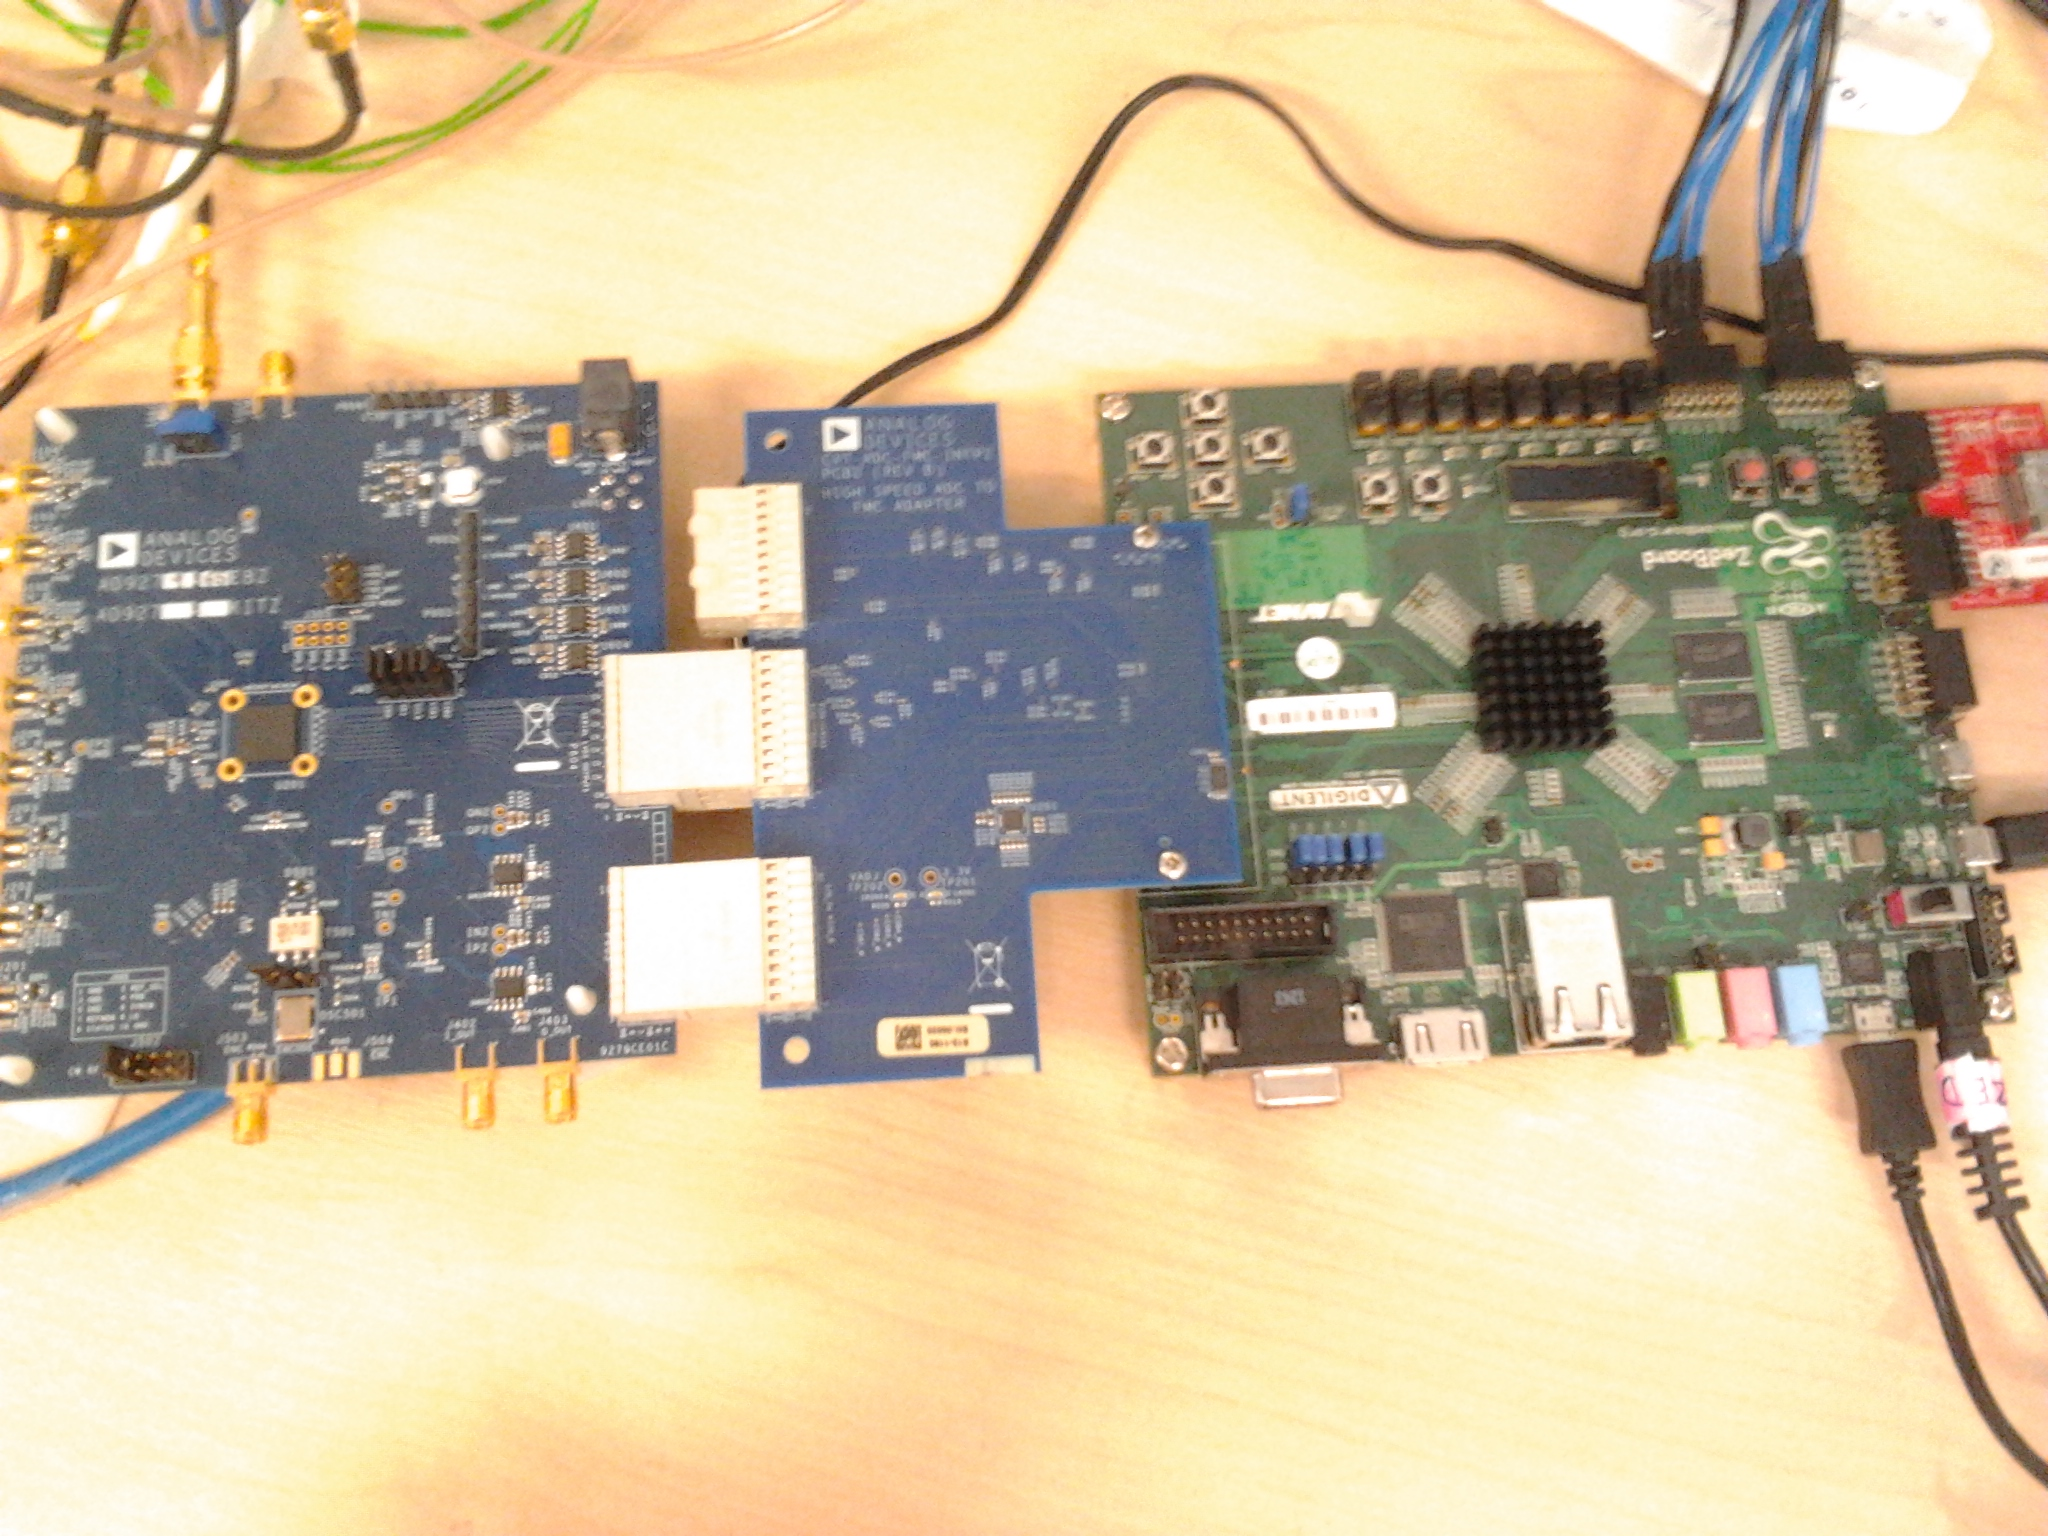
\includegraphics[width=\textwidth]{ad9279}
	\caption{Ο AD9279 (αριστερά) συνδεδεμένος με το Zedboard (δεξιά) μέσω του interposer (μέση)}
	\label{ad9279}
\end{figure}

Η ρύθμιση του ADC γίνεται με τη χρήση του Serial Port Interface (SPI) και πάλι μέσα από το FMC του Zedboard. Μέσω αυτής της θύρας μπορούμε να έχουμε πρόσβαση στους εσωτερικούς registers  του ADC και να αλλάξουμε τιμές στις διάφορες ρυθμίσεις του. Μπορούμε για παράδειγμα να αλλάξουμε τον τερματισμό των σημάτων που στέλνονται προς το FPGA, να αλλάξουμε τον τρόπο αποστολής των δεδομένων από MSB σε LSB ή να δώσουμε εντολή στον ADC να στέλνει γνωστές ακολουθίες ελέγχου (test patterns) αντί για τα κανονικά δεδομένα που ψηφιοποιεί. Αυτή η δυνατότητα είναι πολύ χρήσιμη για τον έλεγχο της ορθής λήψης των δεδομένων από το FPGA.

Τα ψηφιακά σήματα που κατευθύνονται προς το FPGA είναι:
\begin{itemize}
\item ένα διαφορικό σήμα μέσω του οποίου στέλνονται σειριακά τα δεδομένα, για κάθε κανάλι
\item ένα διαφορικό ρολόι για τον συγχρονισμό της λήψης των bits
\item ένα διαφορικό σήμα για την σωστή πλαισίωση (frame) των ληφθέντων bits. Το σήμα αυτό γίνεται ΄1΄ ταυτόχρονα με την αποστολή του 1$ ^{o\upsilon} $ από τα 12 bits.
\end{itemize}

Ένα πρόβλημα που είχαμε με τη χρησιμοποίηση του AD9279 evaluation board με το Zedboard ήταν ότι επειδή το FMC του είναι Low Pin Count, δεν είχαμε πρόσβαση στο frame signal. Χωρίς αυτό δεν μπορεί να γίνει σωστή λήψη των 12 bits  του κάθε sample, αφού δεν είναι γνωστό πιο είναι το 1ο bit ,δηλαδή πού τελειώνει το ένα δείγμα και πού αρχίζει το επόμενο. Αυτή τη δυσκολία όμως μπορέσαμε να την παρακάμψουμε κάνοντας χρήση των test patterns που αναφέρθηκαν προηγουμένως. Συγκεκριμένα, ρυθμίζουμε τον ADC να παράγει ένα συγκεκριμένο και γνωστό test pattern, κάνουμε την ευθυγράμμιση και έπειτα τον ξαναρυθμίζουμε να παράγει κανονικά δεδομένα. Η τεχνική θα αναλυθεί σε επόμενο κεφάλαιο. 

Το πρόβλημα αυτό υπάρχει μόνο κατά τη χρήση της δοκιμαστικής πλακέτας και όχι με την τελική πλακέτα, μιας και αυτή έχει σχεδιαστεί ώστε όλα τα σήματα να περνάνε μέσα από το LPC FMC.


\subsection{MAX4936A evaluation kit}
Ο MAX4936A (εικ. \ref{max4936}) είναι ένας εναλλάκτης (switch) 8 καναλιών για μετάδοση υψηλής τάσης και λήψη χαμηλής τάσης, κατασκευασμένος για χρήση σε εφαρμογές υπερήχων. Έχει προστασία της εξόδου χαμηλής τάσης από την υψηλή τάση που διέρχεται και δυνατότητα απενεργοποίησης κάθε καναλιού ξεχωριστά.
\begin{figure}
	\centering
	
\includegraphics[width=\textwidth]{myimage}
	\caption{MAX4936A evaluation kit}
	\label{max4936}
\end{figure}

Στο πρωτότυπο έχουμε συνδεδεμένη την είσοδο της υψηλής τάσης στις εξόδους των pulsers (MAX4940). Οι παλμοί αυτοί κατευθύνονται στους transducers του phased array για την παραγωγή των υπερήχων. Στη συνέχεια οι transducers λαμβάνουν τις ανακλάσεις και παράγουν ηλεκτρικά σήματα πολύ χαμηλότερης τάσης από τα αρχικά. Αυτά τα σήματα, διέρχονται μέσα από τον switch και κατευθύνονται στον AD9279. Ο switch φροντίζει ώστε οι παλμοί υψηλής τάσης, που κατευθύνονται για τους transducers, να μην διαρρεύσουν προς τον, ευαίσθητο σε τόσο υψηλές τάσεις, AD9279. 




\subsection{Υπολογιστής}
Ο υπολογιστής χρησιμοποιείται για δύο λόγους. Για τον έλεγχο του πρωτοτύπου και για την μετάδοση σε αυτόν των δεδομένων που λαμβάνονται. Τα δεδομένα στη συνέχεια μπορούν να υποστούν επεξεργασία και να απεικονιστούν στην οθόνη. 

Αρχικά η σύνδεση έγινε μέσω της θύρας UART. Η θύρα αυτή είναι πολύ εύκολη στην χρήση, μιας και υπάρχει έτοιμος controller στο Zynq. Επίσης το λογισμικό της Xilinx για τον προγραμματισμό του επεξεργαστή (SDK), κάνει πολύ εύκολη τη χρήση αυτής της θύρας. Το πρόβλημα όμως είναι ότι η σειριακή αυτή θύρα έχει πολύ μικρό bandwidth, το οποίο μπορεί να είναι αρκετό για τον έλεγχο του πρωτοτύπου, αλλά είναι πολύ μικρό για την μετάδοση τον ληφθέντων δεδομένων σε πραγματικό χρόνο.

Για την κάλυψη των αναγκών μας, επιλέχτηκε η λύση του ethernet. Το Zedboard έχει και για αυτό ενσωματωμένο controller, αλλά ο προγραμματισμός της λειτουργίας του είναι πιο περίπλοκος. 

Στην πλευρά του υπολογιστή, για την ανάπτυξη του interface για τον έλεγχο του πρωτοτύπου χρησιμοποιήθηκε το LabVIEW. Η επιλογή του έγινε επειδή επιτρέπει την εύκολη ανάπτυξη γραφικού περιβάλλοντος και έχει έτοιμες συναρτήσεις για την TCP σύνδεση μέσω της ethernet και για την γραφική απεικόνιση των δεδομένων.

\subsection{Τροφοδοτικό υψηλών και χαμηλών τάσεων}
Για την τροφοδοσία των διαφορετικών ολοκληρωμένων κυκλωμάτων θέλουμε μία ποικιλία τάσεων τροφοδοσίας. Για αυτό το λόγο θα χρησιμοποιήσουμε ένα εξειδικευμένο τροφοδοτικό που δίνει τις ακόλουθες τάσεις: $ \pm $1.8V,  $ \pm $3.3V, $ \pm $5V,  +12V, $ \pm $70V.


\section{Απαιτήσεις συστήματος}
Στα επόμενα υποκεφάλαια θα αναλυθούν οι απαιτήσεις που χρειάζεται να καλύπτει το σύστημα που αναπτύξαμε.


\subsection{Ρυθμίσεις συστήματος}
Το σύστημα θα πρέπει να μπορεί να ρυθμίζεται κατά τη διάρκεια της λειτουργίας του, παίρνοντας τις κατάλληλες εντολές από το PS. Πιο συγκεκριμένα θα πρέπει να μπορούμε να ελέγξουμε τα ακόλουθα:
\begin{itemize}
\item Εκκίνηση και σταμάτημα της εκπομπής παλμών και λήψης
\item Μορφή των παραγόμενων παλμών
\item Συχνότητα εκπομπής παλμών (Pulse Repeat Frequency - PRF)
\item Αριθμός δειγμάτων που θα λαμβάνονται μετά από κάθε αποστολή παλμού (και άρα και μέγιστο βάθος στο οποίο το σύστημα μπορεί να ανιχνεύσει
\item Καθυστέρηση έναρξης της λήψης δειγμάτων μετά την αποστολή παλμού
\item Ενεργοποίηση/απενεργοποίηση και έλεγχος του beamforming
\item Έλεγχος του AD9279
\item Ενεργοποίηση και απενεργοποίηση της λειτουργίας του κάθε καναλιού ανεξάρτητα
\end{itemize}

\subsection{Διαμόρφωση δέσμης (Beamforming)}
Όπως αναφέρθηκε νωρίτερα, το σύστημα πρέπει να έχει την ικανότητα διαμόρφωσης δέσμης τόσο κατά την παραγωγή των παλμών υπερήχων, όσο και κατά την λήψη τους. Στη δημιουργία των απαραίτητων καθυστερήσεων (offsets) μεταξύ των παλμών των διαφορετικών καναλιών θα πρέπει να έχει ακρίβεια 3,125 ns και δυνατότητα μέγιστης καθυστέρησης 2μs. Αυτό μας οδηγεί στην χρήση ρολογιού μέγιστης συχνότητας 320 MHz για τους pulsers. Ταυτόχρονα θα πρέπει το σύστημα να μπορεί να πραγματοποιήσει σε πραγματικό χρόνο τη διαμόρφωση δέσμης κατά τη λήψη με μέγιστη συχνότητα δειγματοληψίας τα 80 Msps.


\subsection{Αυτόνομη λειτουργία του συστήματος}
Το σύστημα που σχεδιάσαμε στο FPGA πρέπει να μπορεί να λειτουργεί χωρίς να απασχολεί το PS του Zynq, εκτός φυσικά από τη ρύθμισή του. Αυτό σημαίνει ότι θα πρέπει να μπορεί να στέλνει τα δεδομένα απευθείας στη μνήμη. Άρα θα πρέπει να υπάρχει κάποιο DMA κανάλι. 
Επίσης θα πρέπει να πρέπει να μπορεί να εκτελεί τις διάφορες σαρώσεις κατά το beamforming αυτόνομα. Πριν την έναρξη κάθε ακολουθίας ο επεξεργαστής θα δίνει στο σύστημα το πλήθος των βημάτων καθώς και τη διεύθυνση στην οποία βρίσκονται οι ρυθμίσεις για όλα τα βήματα. Στη συνέχεια το σύστημα θα πρέπει να έχει πρόσβαση στη μνήμη, από όπου θα ανακτάει τις κατάλληλες ρυθμίσεις πριν από κάθε βήμα. 

\subsection{Απαιτήσεις μνήμης και εύρος διαύλων μεταφοράς δεδομένων}
Ο ανιχνευτής θα πρέπει να έχει την ικανότητα να απεικονίσει μία περιοχή με μέγιστο βάθος 10 εκατοστών ενός μεταλλικού αντικειμένου. Ξέροντας ότι η ταχύτητα του ήχου στο σίδερο είναι 5900m/s υπολογίζουμε ότι οι παλμοί υπερήχων για να φτάσουν σε αυτό το βάθος και να επιστρέψουν στους αισθητήρες θέλουν 34 μs. Για συχνότητα δειγματοληψίας 80 Msps αυτό μας δίνει περίπου 2700 δείγματα. Το κάθε δείγμα είναι 12 bits, αλλά για λόγους σωστής στοίχισης των δειγμάτων με τις θέσεις μνήμης, αναγκαζόμαστε να τα χειριζόμαστε ως 16 bits. Βλέπουμε λοιπόν ότι έχουμε 5,4kB ανά κανάλι. Δηλαδή για τα 8 κανάλια έχουμε 43,2kB. Για μέγιστο PRF 100Hz έχουμε 4,2MB/s ή 33,75Mb/s.

Θα χρησιμοποιήσουμε την DDR3 RAM που υπάρχει πάνω στο Zedboard, ώστε να έχουμε αρκετό αποθηκευτικό χώρο για να αποθηκεύουμε τα δεδομένα. Επίσης από από εκεί μπορούμε να τα εύκολα να τα επεξεργαστούμε με τον επεξεργαστή, ώστε να εμφανίσουμε την απεικόνισή τους στην οθόνη αφής ή να τα στείλουμε στον υπολογιστή μέσω της ethernet. 

Ο controller της DDR μπορεί να μεταφέρει μέχρι και 4,2GB/s και οι High Performance AXI ports είναι ακόμα πιο γρήγορες. Άρα βλέπουμε ότι η ταχύτητα μεταφοράς των δεδομένων στη μνήμη δεν θα μας δημιουργήσει πρόβλημα.


\chapter{Σχεδιασμός και υλοποίηση του συστήματος}
Η υλοποίηση του συστήματος πρέπει να πραγματοποιηθεί σε 4 διαφορετικά στάδια. Το κάθε ένα από τα στάδια αυτά αναπτύχθηκαν με διαφορετικά εργαλεία και μεθόδους. Στις επόμενες παραγράφους θα αναπτυχθούν τα στάδια αυτά, ξεκινώντας από το πιο ειδικό και καταλήγοντας στο πιο γενικό, και θα παρουσιαστούν κάποιες σχεδιαστικές αποφάσεις που πάρθηκαν καθώς και τα εργαλεία που χρησιμοποιήθηκαν. 

\section{Στάδια σχεδιασμού}
\subsection{Σχεδιασμός του πυρήνα παραγωγής παλμών και λήψης δεδομένων}
Αυτό το στάδιο είναι το πιο βασικό, καθώς περιλαμβάνει το σχεδιασμό του πυρήνα του συστήματός μας με την ονομασία AXI pulser receiver. Από αυτόν παράγονται τα σήματα που οδηγούν την παραγωγή των παλμών υψηλής τάσης από τους pulsers Επίσης εδώ καταλήγουν τα ψηφιακά δεδομένα από τον ADC. Τα δεδομένα αυτά μετατρέπονται από σειριακά σε παράλληλα. Έπειτα, στην περίπτωση που έχουμε επιλέξει την λειτουργία beamforming, γίνονται οι όποιοι υπολογισμοί και τέλος μετατρέπονται σε μία ροή δεδομένων (data stream) έτοιμα για να σταλούν στη μνήμη.

Για το σχεδιασμό του χρησιμοποιήθηκε η γλώσσα περιγραφής υλικού VHDL στο softaware VIvado της Xilinx. Κατά τη διάρκεια του σχεδιασμού είχαμε δύο βασικές αρχές. Το σύστημα να είναι όσο το δυνατόν πιο παραμετροποιημένο με τη χρήση generics παραμέτρων. Ειδικά όσο αναφορά τον αριθμό των καναλιών. Αυτό είναι σημαντικό, για την εύκολη επαναχρησιμοποίηση σε συστήματα με περισσότερα κανάλια, κάτι που είναι εξαρχής το στόχος της ανάπτυξης του πρωτοτύπου. 

Ταυτόχρονα οι όποιες θύρες επικοινωνίας υπάρχουν θα πρέπει να είναι συμβατές με το πρότυπο AXI. Το πρότυπο αυτό έχει πολύ ευρεία χρήση και δίνει μεγάλη ευκολία σύνδεσης μεγάλου πλήθους διαφορετικών μονάδων, χωρίς την ανάγκη κατανόησης της εσωτερικής λειτουργίας τους. Επίσης η χρήση του προτύπου επιτρέπει τη σύνδεση με όλα τα έτοιμα περιφερειακά που προσφέρει η Xilinx καθώς και με την PS πλευρά του Zynq.

Πιο συγκεκριμένα το core έχει τα παρακάτω interfaces:
\begin{enumerate}
\item \textbf{Slave AXI lite:} Συνδέεται με τον επεξεργαστή και του δίνει πρόσβαση στους εσωτερικούς καταχωρητές του core. Με αυτόν τον τρόπο ο επεξεργαστής έχει έλεγχο όλων των ρυθμίσεών του.
\item \textbf{Master AXI full:} Συνδέεται απευθείας με τη DDR και επιτρέπει στο core να διαβάζει, όποτε τα χρειάζεται, τα απαραίτητα δεδομένα για το beamforming. Επιλέχτηκε το full interface αντί του lite επειδή δίνει τη δυνατότητα για burst mode read, που είναι πολύ χρήσιμο για τη γρήγορη πρόσβαση στα δεδομένα
\item\textbf{Master AXI Stream:} Από εδώ εξέρχονται τα δεδομένα που έχουν ληφθεί από τον ADC μετά την όποια επεξεργασία. 
\end{enumerate}

Μετά το τέλος της υλοποίησης του πυρήνα, τον πακετάραμε ως IP core για τη χρήση στον IP intergrator στο επόμενο στάδιο της ανάπτυξης.


\subsection{Σχεδιασμός του συστήματος}
Για τον σχεδιασμό ολόκληρου του συστήματος, μέσα στο οποίο ενσωματώθηκε το IP core AXI pulser receiver, χρησιμοποιήθηκε ο IP intergrator του Vivado. Σε αυτό το στάδιο πραγματοποιήθηκε η σύνδεση του core με τη μνήμη και τον επεξεργαστή, με τη βοήθεια κάποιων άλλων έτοιμων cores της Xilinx. Προστέθηκαν ακόμα με τον κατάλληλο τρόπο τα cores που συνόδευαν την οθόνη αφής.

\subsection{Προγραμματισμός του επεξεργαστή}
Σε αυτό το στάδιο πραγματοποιήσαμε τον προγραμματισμό του επεξεργαστή. Ο προγραμματισμός έγινε στο SDK της Xilinx σε γλώσσα C. Υπάρχουν δύο επιλογές για τον τρόπο λειτουργίας του επεξεργαστή. Ο πρώτος είναι η φόρτωση ενός ολοκληρωμένου λειτουργικού συστήματος linux, έτοιμο και κατάλληλα παραμετροποιημένο για τον συγκεκριμένο επεξεργαστή από την Xilix και η δημιουργία εφαρμογής που θα τρέχει κάτω από αυτό το λειτουργικό. Η δεύτερη επιλογή είναι η δημιουργία εφαρμογής που θα τρέχει χωρίς την απαίτηση για ολοκληρωμένο λειτουργικό σύστημα, αναφερόμενη και ως baremetal application. Επιλέξαμε τη δεύτερη επιλογή, για να μην φορτώσουμε τον επεξεργαστή με την εκτέλεση ολόκληρου λειτουργικού και για να έχουμε καλύτερο έλεγχο της λειτουργίας του. Από την άλλη, αυτό σημαίνει ότι ο προγραμματισμός είναι πιο χαμηλού επιπέδου και πιο δύσκολος. 

Οι λειτουργίες της εφαρμογής είναι ο έλεγχος του AXI pulser receiver, η αποστολή των δεδομένων μέσω του ethernet στον υπολογιστή, η λειτουργίας της οθόνης αφης και η απεικόνιση των δεδομένων σε αυτή.


\section{Υλοποίηση του συστήματος}

Σε αυτό το κεφάλαιο θα παρουσιάσουμε αναλυτικά τα στάδια υλοποίησης του συστήματος που αναφέρθηκαν στο προηγούμενο κεφάλαιο. 

\subsection{AXI pulser receiver}

\subsubsection{Επισκόπηση}
Ο πυρήνας αυτός είναι σύστημα για τη δημιουργία παλμών υπερήχων και τη λήψη δεδομένων από τον ADC και μετατροπή τους σε Master AXI stream κατάλληλο για τη σύνδεση με οποιοδήποτε Slave AXI stream interface. Αυτό δίνει τη δυνατότητα για σύνδεση με οποιοδήποτε στοιχείο μνήμης, ανεξάρτητα από το είδος και τον τρόπο λειτουργίας της, αρκεί αυτή να υπακούει στο AXI πρότυπο. Στο διάγραμμα \ref{axi_pr_block} βλέπουμε τη δομή του core.

Το AXI-lite interface χρησιμοποιείται για τον προγραμματισμό των registers την μονάδας ελέγχου. Στη συνέχεια, η μονάδα ελέγχου ελέγχει τα επιμέρους στοιχεία του συστήματος, ανάλογα φυσικά με τον προγραμματισμό που της έχουμε κάνει.

Το AXI full interface συνδέεται σε μνήμη μέσα στην οποία είναι αποθηκευμένα τα δεδομένα που είναι απαραίτητα για το beamforming.

\begin{figure}
	\centering
	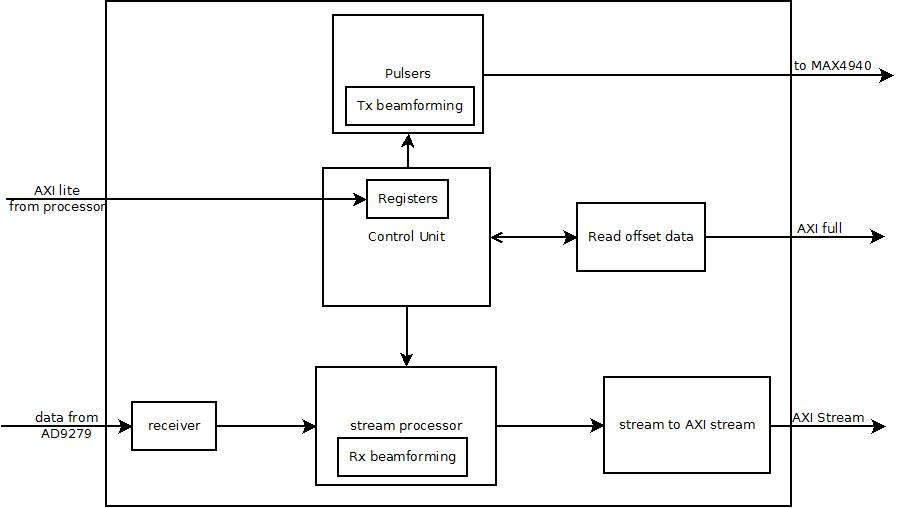
\includegraphics[width=\textwidth]{axi_pr_block}
	\caption{AXI pulser receiver μπλοκ διάγραμμα}
	\label{axi_pr_block}
\end{figure}



\subsubsection{Register map}



\subsubsection{Control Unit}
Το Control Unit (CU) αποτελεί τον εγκέφαλο του συστήματος, μιας και κατευθύνει τα υπόλοιπα μέρη του συστήματος. Αποτελείται από αρκετούς registers, μέσω των οποίων γίνεται η επικοινωνία με τον επεξεργαστή, και από ένα Finite State Machine. Το FSM καθορίζει τη σειρά λειτουργίας των επιμέρους συστημάτων και φροντίζει για τον συγχρονισμό τους.



\subsubsection{Pulser}
O pulser λειτουργεί με το δικό του ρολόι και αναλαμβάνει τη δημιουργία των σημάτων που θα σταλούν στον MAX4940, αμέσως μόλις του δοθεί σήμα από το control unit. Η μορφή των σημάτων καθορίζεται από τα μοτίβα που δέχεται από το control unit. Τα patterns αυτά είναι 32bits και τροφοδοτούνται σε shift registers. Η συχνότητα με την οποία ολισθαίνουν οι registers καθορίζεται από το port freq-divider. 

Ταυτόχρονα, ο Pulser  αναλαμβάνει την καθυστέρηση των σημάτων, ανάλογα με το offset που του στέλνεται από το CU. Στον πίνακα \ref{pulser_generics} μπορούμε να δούμε τις generic παραμέτρους και στον πίνακα \ref{pulser_ports} τα ports καθώς και την περιγραφή τους.

\begin{table}
\center
\begin{tabular}{|l|r|}
\hline 
Όνομα & Τιμή \\ 
\hline 
PATTERN\_BITS & 32 \\ 
\hline 
OFFSET\_BITS & 10 \\ 
\hline 
FREQ\_DIV\_BITS & 4 \\ 
\hline 
\end{tabular} 
\caption{Pulser Generic Paramaters}
\label{pulser_generics} 
\end{table} 


\begin{table}
\begin{tabularx}{\linewidth}{|l|c|c|X|}
\hline 
Όνομα & Κατεύθυνση & Πλάτος & Περιγραφή \\ 
\hline 
\hline 
pulser\_clk & in & 1 & Το ρολόι λειτουργίας της μονάδας \\ 
\hline 
freq\_divider & in & FREQ\_DIV\_BITS & Ο αριθμός των περιόδων του ρολογιού που πρέπει να διαρκεί κάθε βήμα των patterns \\ 
\hline 
pulse\_synq\_in & in & 1 & Σήμα για την εκκίνηση της παραγωγής του παλμού \\ 
\hline 
p\_pattern\_in & in & PATTERN\_BITS & Pattern για την παραγωγή του θετικού πόλου του παλμού \\ 
\hline 
clamp\_pattern\_in & in & PATTERN\_BITS & Pattern για την επιστροφή στο μηδέν του παλμού \\ 
\hline 
n\_pattern\_in & in & PATTERN\_BITS & Pattern για την παραγωγή του αρνητικού πόλου του παλμού \\ 
\hline 
offset\_in & in & OFFSET\_BITS & Καθυστέρηση για την παραγωγή του παλμού από τη στιγμή που ληφθεί το σήμα pulse\_synq\_in, σε περιόδους του ρολογιού \\ 
\hline 
pulse\_out\_en & out & 1 & Το απαραίτητο για τη λειτουργία του MAX4940, enable \\ 
\hline 
pulse\_out\_p & out & 1 & Ο θετικός πόλος του παλμού \\ 
\hline 
pulse\_out\_clam & out & 1 & Σήμα για την επιστροφή στο μηδέν \\ 
\hline 
pulse\_out\_n & out & 1 & Ο αρνητικός πόλος του παλμού \\ 
\hline 
pulsing\_out & out & 1 & Σήμα ότι η μονάδα λειτουργεί \\ 
\hline 
\end{tabularx} 
\caption{Pulser Ports description}
\label{pulser_ports} 
\end{table} 